% ----------------------------------------------------------------
%       Speech Signal Processing Toolkit (SPTK): version 3.0
%                      SPTK Working Group
% 
%                Department of Computer Science
%                Nagoya Institute of Technology
%                             and
%   Interdisciplinary Graduate School of Science and Engineering
%                Tokyo Institute of Technology
%                   Copyright (c) 1984-2000
%                     All Rights Reserved.
% 
% Permission is hereby granted, free of charge, to use and
% distribute this software and its documentation without
% restriction, including without limitation the rights to use,
% copy, modify, merge, publish, distribute, sublicense, and/or
% sell copies of this work, and to permit persons to whom this
% work is furnished to do so, subject to the following conditions:
% 
%   1. The code must retain the above copyright notice, this list
%      of conditions and the following disclaimer.
% 
%   2. Any modifications must be clearly marked as such.
%                                                                        
% NAGOYA INSTITUTE OF TECHNOLOGY, TOKYO INSITITUTE OF TECHNOLOGY,
% SPTK WORKING GROUP, AND THE CONTRIBUTORS TO THIS WORK DISCLAIM
% ALL WARRANTIES WITH REGARD TO THIS SOFTWARE, INCLUDING ALL
% IMPLIED WARRANTIES OF MERCHANTABILITY AND FITNESS, IN NO EVENT
% SHALL NAGOYA INSTITUTE OF TECHNOLOGY, TOKYO INSITITUTE OF
% TECHNOLOGY, SPTK WORKING GROUP, NOR THE CONTRIBUTORS BE LIABLE
% FOR ANY SPECIAL, INDIRECT OR CONSEQUENTIAL DAMAGES OR ANY
% DAMAGES WHATSOEVER RESULTING FROM LOSS OF USE, DATA OR PROFITS,
% WHETHER IN AN ACTION OF CONTRACT, NEGLIGENCE OR OTHER TORTIOUS
% ACTION, ARISING OUT OF OR IN CONNECTION WITH THE USE OR
% PERFORMANCE OF THIS SOFTWARE.
% ----------------------------------------------------------------
%
\hypertarget{fftr2}{}
\name{fftr2}{2-dimensional FFT for real sequence}{signal processing}

\begin{synopsis}
\item[fftr2] [ --l $L$ ] [ --m $M_1 \; M_2$ ] [ --t ] [ --c ] [ --q ] 
	     [ --\{ A $|$ R $|$ I $|$ P \} ] [ {\em infile} ] 
\end{synopsis}

\begin{qsection}{DESCRIPTION}
{\em fftr2} uses the 2-dimensional Fast Fourier Transform (FFT) algorithm 
to calculate the 2-dimensional Discrete Fourier Transform (DFT) 
of real-valued input data from {\em infile} (or standard input), 
sending the result to standard output. 
The input and output data is in float format, arranged as follows.
\begin{center}
 \leavevmode
 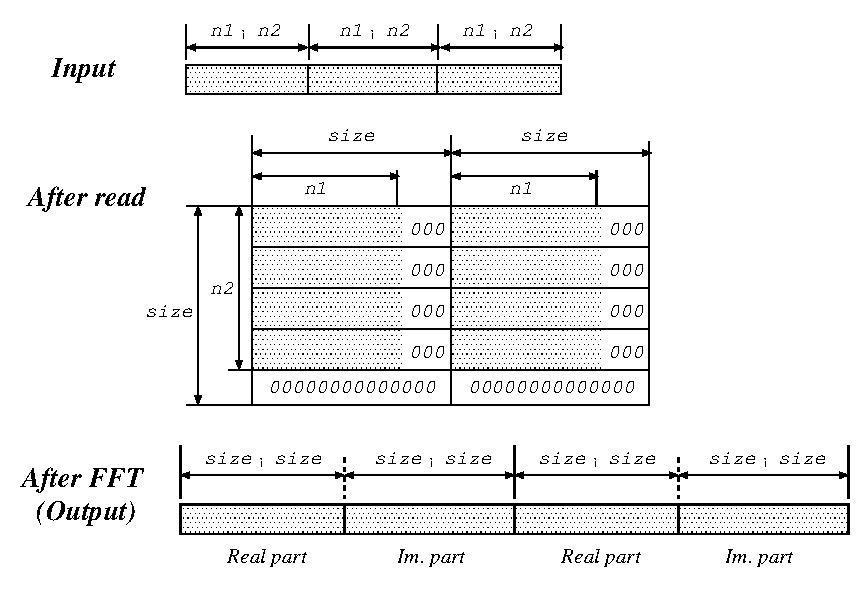
\includegraphics{fig/fftr2.eps}
\end{center}
\end{qsection}

\begin{options}
	\argm{l}{L}{FFT size  power of 2}{64}
	\argm{m}{M_1 \; M_2}{order of sequence ($M_1\times M_2$).
			If the file size $k$ is smaller than $64^2$
			and $\sqrt{k}$ is integer value, $M_1=M_2=\sqrt{k}$. 
			Otherwise output error message to standard error output 
			and then terminate.}{$64 , M_1$}
	\argm{t}{}{Output results in transposed form (see also \hyperlink{fft2}{fft2}).}{FALSE}
	\argm{c}{}{When results are transposed, 1 boundary data is copied from the
	opposite side, and then output $(L+1)\times (L+1)$ data (see also \hyperlink{fft2}{fft2}).}{FALSE}
	\argm{q}{}{Output first $1/4$ data of FFT results only.
		   As in the above c option, boundary data is compensated and 
		   $(\frac{L}{2}+1)\times(\frac{L}{2}+1)$ data are output
		   (see also \hyperlink{fft2}{fft2}).}{FALSE}
	\argm{A}{}{amplitude}{FALSE}
	\argm{R}{}{real part}{FALSE}
	\argm{I}{}{imaginary part}{FALSE}
	\argm{P}{}{output power spectrum}{FALSE}
\end{options}

\begin{qsection}{EXAMPLE}
This example reads a sequence of 2-dimensional real numbers in float format
from {\em data.f} file, evaluates its 2-dimensional DFT and outputs it to {\em
data.dft} file:
\begin{quote}
  \verb!fftr2 -A data.f > data.dft!
\end{quote}
\end{qsection}

\begin{qsection}{SEE ALSO}
\hyperlink{fft}{fft},
\hyperlink{fft2}{fft2},
\hyperlink{ifft}{ifft}
\end{qsection}
